\documentclass[a4paper, 11pt]{article} %option para: draft mode not insert figure, give a faster preview
\usepackage[UTF8]{ctex} %for chinese
\usepackage{amsmath}    %for math
\usepackage{geometry}   %for page setting
\usepackage{graphicx}   % for insert graph
\usepackage{color}    %for link and code color
\usepackage{float}    %for graph table in the follow word
\usepackage[colorlinks,linkcolor=blue,anchorcolor=blue,citecolor=green]{hyperref} %for a linked ref

\setlength{\parindent}{2em} % maybe not use delete it ?
\geometry{left=3.0cm, right=3.0cm, top=3.0cm, bottom=3.0cm}

\graphicspath{{figure/}}


%%%%%%%%%%%%%%%%%%%%%%%%%%%%%%%%%%%%%%%%%%%%%%%%%%%%%%%%%%%%%%%%%%%%%%%%%%%%%%%%%%%%%%%%%%%%%%
%%%%             optional package default in comment to improve compile speed            %%%%

% \usepackage{physics}    %for a readable formulation


% \usepackage[all]{hypcap} % use to jump to the top of figure/table rather than merely caption

% \usepackage{fancyhdr}
% \pagestyle{fancy} % leftmark is a build-in marco means the current higher level in markboth, right is a lower one

% \addtolength{\headheight}{\baselineskip} % use to delete headheight waring
% \fancyfoot[C]{\thepage}
% \fancyhead[L]{\leftmark}
% \fancyhead[R]{\rightmark}
% \renewcommand{\headrulewidth}{0pt}
% \pagestyle{fancy}

\usepackage[final]{listings} %for code use final to exclude draft mode to show whenever it is
\definecolor{dkgreen}{rgb}{0,0.6,0}
\definecolor{gray}{rgb}{0.5,0.5,0.5}
\definecolor{mauve}{rgb}{0.58,0,0.82}

\lstset{frame=tb,
  language=c++,
  aboveskip=3mm,
  belowskip=3mm,
  showstringspaces=false,
  columns=flexible,
  basicstyle={\small\ttfamily},
  numbers=left, %none, right
  numberstyle=\tiny\color{gray},
  keywordstyle=\color{blue},
  commentstyle=\color{dkgreen},
  stringstyle=\color{mauve},
  breaklines=true,
  breakatwhitespace=true,
  tabsize=2,
  captionpos=b
}
\renewcommand{\lstlistingname}{源代码} % to change the prefix as 源码 not Listing
\renewcommand{\lstlistlistingname}{源代码} % header name in list of listing
% \usepackage{fontspec}
% \setmonofont{Consolas} % set consolas in coding box, ONLY XeLaTeX so default comment remember a fontspec only used at the following


% \usepackage{wrapfig}  % for picutre on the paragraph right, cannot work with chinese par in pdflatex


% % \usepackage{fontspec} % for other font family


% \usepackage{multirow} %for group row in a table


% % Threeparttable
% \usepackage{threeparttable}
% \usepackage{booktabs}


% % drawing script tikz and Circuitlib 
% \usepackage{tikz}
% \usetikzlibrary{circuits.ee.IEC}
% \usetikzlibrary{positioning}

% \usepackage[american]{circuitikz}

%%%%%%%%%%%%%%%%%%%%%%%%%%%%%%%%%%%%%%%%%%%%%%%%%%%%%%%%%%%%%%%%%%%%%%%%%%%%%%%%%%%%%%%
%%%%%                         new recommand setting area                           %%%%

% % Count those in subsection
% \makeatletter
% \@addtoreset{equation}{subsection}
% \@addtoreset{figure}{subsection}
% \@addtoreset{table}{subsection}
% \makeatother
% \renewcommand {\thefigure} {\thesubsection{}.\arabic{figure}}
% \renewcommand {\thetable} {\thesubsection{}.\arabic{table}}
% \renewcommand {\theequation} {\thesubsection{}.\arabic{equation}}


% \newcommand{\parallelsum}{\mathbin{\!/\mkern-5mu/\!}} % parallesum for resistor
% \newcommand{\upcite}[1]{\textsuperscript{\textsuperscript{\cite{#1}}}}

%%%%%%%%%%%%%%%%%%%%%%%%%%%%%%%%%%%%%%%%%%%%%%%%%%%%%%%%%%%%%%%%%%%%%%%%%%%%%%%%%%%%%%
%%%%%%%%%%%%%%%%%%%%%%%%              for a dairy box%          %%%%%%%%%%%%%%%%%%%%%%

%%%%%%%%%%%%%%%%%%%%%%%%%%%%%%%%%%%%%%%%%%%%%%%%%%%%%%%%%%%%%%%%%%%%%%%%%%%%%%%%%%%%%%%
%%%%%                         introduction section area                           %%%%

\usepackage{xcolor}
\usepackage{framed}


\newlength\sidebar
 \newlength\envrule
 \newlength\envborder
 \setlength\sidebar{1.5mm}
 \setlength\envrule{0.4pt}
 \setlength\envborder{2mm}

\makeatletter
 \long\def\fboxs#1{%
   \leavevmode
   \setbox\@tempboxa\hbox{%
     \color@begingroup
       \kern\fboxsep{#1}\kern\fboxsep
     \color@endgroup}%
   \@frames@x\relax}
 \def\frameboxs{%
   \@ifnextchar(%)
     \@framepicbox{\@ifnextchar[\@frameboxs\fboxs}}
 \def\@frameboxs[#1]{%
   \@ifnextchar[%]
     {\@iframeboxs[#1]}%
     {\@iframeboxs[#1][c]}}
 \long\def\@iframeboxs[#1][#2]#3{%
   \leavevmode
   \@begin@tempboxa\hbox{#3}%
     \setlength\@tempdima{#1}%
     \setbox\@tempboxa\hb@xt@\@tempdima
          {\kern\fboxsep\csname bm@#2\endcsname\kern\fboxsep}%
     \@frames@x{\kern-\fboxrule}%
   \@end@tempboxa}
 \def\@frames@x#1{%
   \@tempdima\fboxrule
   \advance\@tempdima\fboxsep
   \advance\@tempdima\dp\@tempboxa
   \hbox{%
     \lower\@tempdima\hbox{%
       \vbox{%
        \hrule\@height\fboxrule
       %  \hbox{%
        %  \vrule\@width\fboxrule

           #1%
           \vbox{%
             \vskip\fboxsep
             \box\@tempboxa
             \vskip\fboxsep}%
           #1%
           }\vrule\@width\fboxrule}%
         }%\hrule\@height\fboxrule}%
                          % }%
        % }%
 }
 \def\esefcolorbox#1#{\esecolor@fbox{#1}}
 \def\esecolor@fbox#1#2#3{%
   \color@b@x{\fboxsep\z@\color#1{#2}\fboxs}{\color#1{#3}}}
 \makeatother


 \definecolor{exampleborder}{HTML}{00CED1}
 \definecolor{examplebg}{HTML}{CEF6EC}
 \definecolor{statementborder}{rgb}{.9,0,0}
 \definecolor{statementbg}{rgb}{255,255,255}

 \newenvironment{eseframed}{%
   \def\FrameCommand{\fboxrule=\the\sidebar  \fboxsep=\the\envborder%
   \esefcolorbox{exampleborder}{examplebg}}%
   \MakeFramed{\FrameRestore}}%
  {\endMakeFramed}


 \newcounter{diary}
\renewcommand{\thediary}{\arabic{diary}}

 %%% CODE ENVIRONMENT. PUT TEXT INTO COLORED FRAME %%%
 \newenvironment{diary}[2]
 {\par\medskip\refstepcounter{diary}%
 \hbox{%
 \fboxsep=\the\sidebar\hspace{-\envborder}\hspace{-0.5\sidebar}%
 \colorbox{exampleborder}{%
 \hspace{\envborder}\footnotesize\sffamily\bfseries%
 \textcolor{black}{{#1}\ {#2}\enspace\hspace{\envborder}}
%\today
 }
 }
 \nointerlineskip\vspace{-\topsep}%
 \begin{eseframed}\noindent\ignorespaces%
 }
 {\end{eseframed}\vspace{-\baselineskip}\medskip}

\begin{document}

\begin{diary}{}{2019.07.01上午}

电子设计小学期工作日的第一个上午,首先我们较为顺利地通过了预习验收,鼓舞了项目开始时的士气。

此外,在等待验收的前前后后的过程中,我们主要使用\href{https://www.w3cschool.cn/arduino/}{W3Cschool的arduino教程},对我们所选的主控模块进行了简单的上手热身。主要了解了其整体的程序语法,控制流,IO功能和串口通信调试功能。

接近上午调试结束时,我们还盘点了已有的一些模块。我们现有的模块有LCD显示屏,蓝牙通信模块,基本可以实现数字部分的功能。而模拟部分的模块,大部分传感器仍在配送,电源管理模块可先根据已有的备选芯片进行一定的调试。故而我们敲定了之后的计划,按照电源管理、arduino并行的方法进行调试。而LCD的调试相蓝牙模块调试调试而言比较简单,故先进行调试;并且另一路对电源管理模块调试的结束后,可以分人手去提前学习一下蓝牙模块的使用。得到近期调试优先度大纲如下:

\begin{enumerate}
  \item arduino,LCD,串口联调;电源管理模块参数测试
  \item 蓝牙模块学习调试。
  \item 传感器模块的参数调试与联调。
  \item 其他基于分立元件(如光敏电阻)的外围传感电路设计
  \item 写数字系统整体代码框架
\end{enumerate}

\end{diary}

\begin{diary}{}{2019.07.01下午}

\par{}在经过上午的验收以及上手热身后,我们在下午正式开启了设计与调试,由于大多数传感器还没有送达,我们手中已有的模块是arduino uno主控模块和LCD1602液晶显示模块,为了减少IO的使用,我们特地前往中发电子大厦购买了I2C转接板,将16引脚方便的减少为4引脚和arduino相连接。

在购置回转接板后,我们一方面开始学习LCD1602与arduino的硬件连接方法,以及其各个引脚的说明,并且在利用已有的LiquidCrystal库函数的情况下,尝试进行了字符数据的显示,成果如下:
\begin{figure}[H]
  \centering
  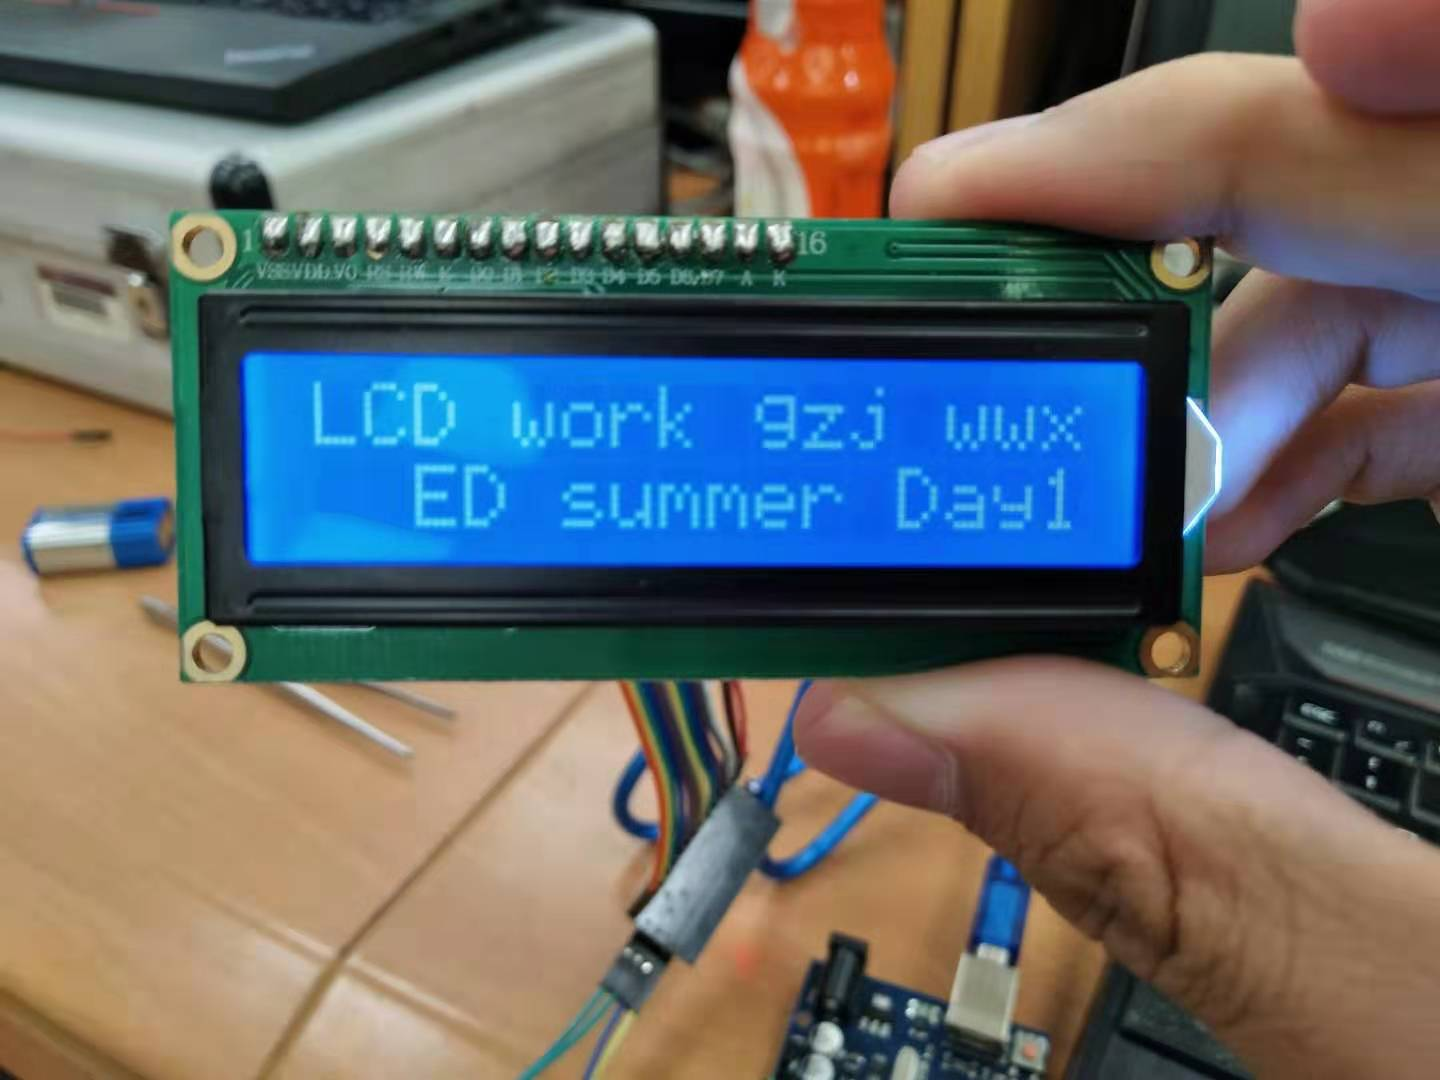
\includegraphics[width = 0.53\textwidth]{chuan2.jpg}
  \caption{LCD字符显示}
\end{figure}
起初并不能显示,后来我们很快发现是转接板电位器的问题,转接板电位器直接控制了LCD显示的亮度,因此在使用镊子改变电位到合适的亮度后便能观察到字符。在能够显示字符后,我们进一步结合上午的学习进行了串口LCD通信联调,使得在键盘上实时输入字符在LCD上进行显示,这是我们之后显示模块的重要基础,我们拍摄成果的照片如下:
\begin{figure}[H]
  \centering
  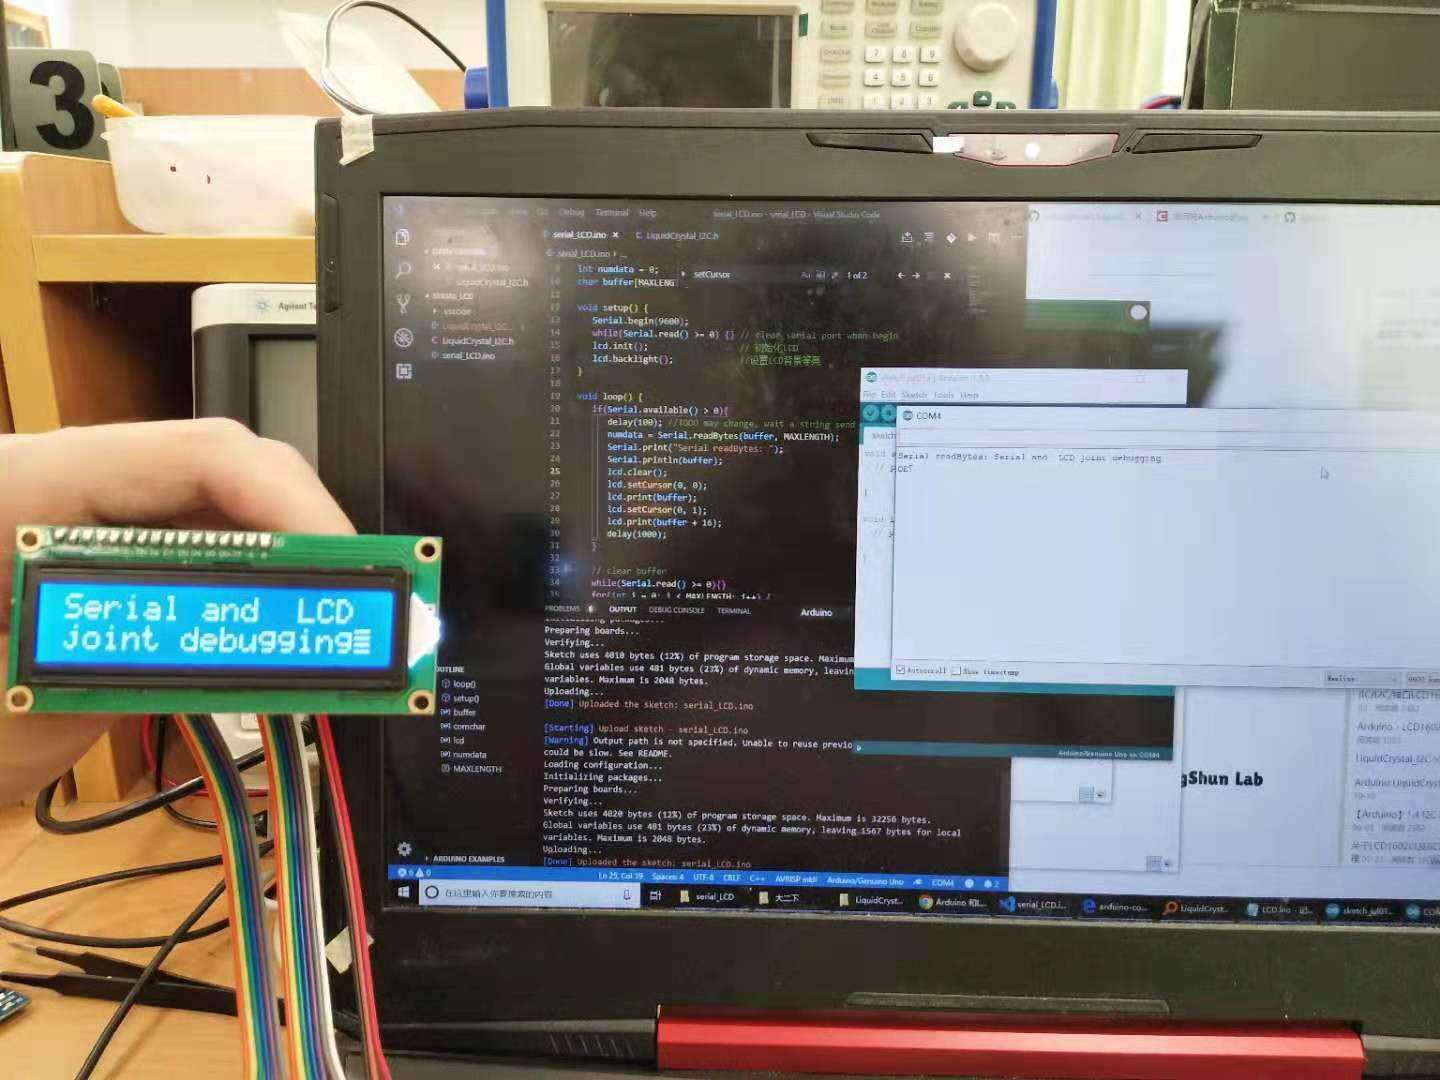
\includegraphics[width = 0.53\textwidth]{chuan1.jpg}
  \caption{LCD串口通信联调}
\end{figure}
另一方面,我们组在调试LCD的同时,对电源管理电路进行了实际的检测,我们计划使用9V的干电池,而恰好在实验室中找到一块电源管理的模块,能够在小于12V输入的情况下,输出5V/3.3V的直流电压,我们类比于电网$10\%$的波动,使用$8V\sim 10V$的50Hz正弦波作为输出,观察两输出的电压情况,结果十分令人满意,根据示波器的显示,以及自动测量的结果,能够得到纹波非常小的直流电压,并十分接近其标称的输出,记录如下图所示:
\begin{figure}[H]
  \begin{minipage}[t]{0.45\linewidth}
      \centering
      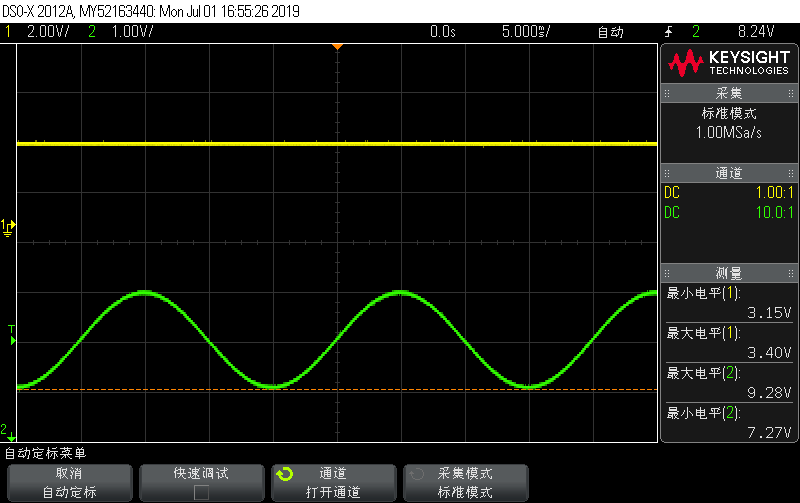
\includegraphics[width=6cm]{dy1.png}
      \caption{3.3V稳压输出}
  \end{minipage}%
      \hfill
  \begin{minipage}[t]{0.45\linewidth}
      \centering
      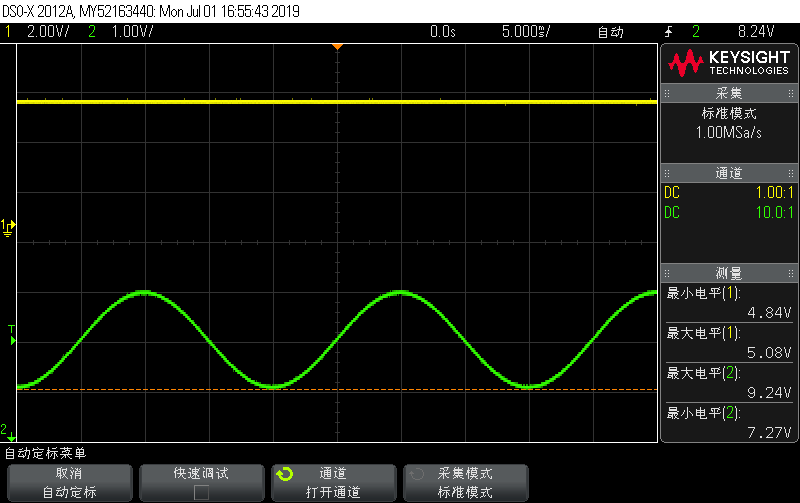
\includegraphics[width=6cm]{dy2.png}
      \caption{5V稳压输出}
  \end{minipage}
\end{figure}
其中黄色线为稳压输出,绿色线为输入,验证了该电源管理模块能够提供理想的供电电压,在TI公司的样片到来之前为我们的电源管理提供了替代。

在下午收工以后我们另外找到一片蓝牙模块,计划于明天开启蓝牙模块的调试以及DHT11的湿度模块的调试,并通过LiquidCrystal库编写代码,实现自己需要的函数的头文件。

\end{diary}
\end{document}
